\documentclass[tikz,border=3pt]{standalone}

\usepackage{lmodern}
\usetikzlibrary{arrows.meta,decorations.markings}

\definecolor{phononblue}{RGB}{31,119,180}

\begin{document}
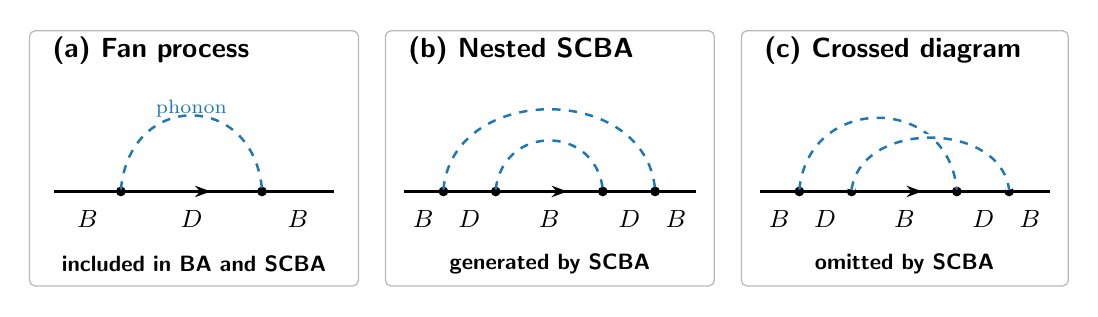
\begin{tikzpicture}[
  % Native width matches a 0.75-linewidth SI inclusion, so the text is not
  % reduced a second time by LaTeX.
  x=0.8cm,
  y=0.8cm,
  font=\sffamily\footnotesize,
  matter/.style={
    draw=black,
    line width=0.85pt,
    postaction={decorate},
    decoration={markings,mark=at position 0.56 with
      {\arrow{Stealth[length=2.0mm,width=1.45mm]}}}
  },
  phonon/.style={draw=phononblue,dashed,line width=0.9pt},
  crossingphonon/.style={
    phonon,
    preaction={draw=white,solid,line width=2.6pt}
  },
  vertex/.style={circle,fill=black,inner sep=1.25pt},
  panel/.style={draw=black!28,rounded corners=2pt,line width=0.45pt},
  paneltitle/.style={anchor=west,font=\sffamily\bfseries\normalsize},
  state/.style={font=\sffamily\small},
  verdict/.style={font=\sffamily\footnotesize\bfseries,text=black}
]

% Keep an explicit, stable bounding box for reproducible inclusion in the SI.
\path[use as bounding box] (0,0) rectangle (16.55,4.15);

% --------------------------------------------------------------------------
% (a) Leading bright--dark--bright Fan channel.
% --------------------------------------------------------------------------
\begin{scope}
  \draw[panel] (0.03,0.05) rectangle (5.25,4.10);
  \node[paneltitle] at (0.24,3.78) {(a) Fan process};

  \draw[matter] (0.42,1.55)--(4.86,1.55);
  \node[vertex] at (1.48,1.55) {};
  \node[vertex] at (3.72,1.55) {};
  \draw[phonon]
    (1.48,1.58) .. controls (1.62,3.15) and (3.58,3.15) .. (3.72,1.58);
  \node[text=phononblue,font=\scriptsize] at (2.60,2.86) {phonon};

  \node[state] at (0.95,1.12) {$B$};
  \node[state] at (2.60,1.12) {$D$};
  \node[state] at (4.29,1.12) {$B$};
  \node[verdict] at (2.64,0.40)
    {included in BA and SCBA};
\end{scope}

% --------------------------------------------------------------------------
% (b) The nested noncrossing O(g^4) repetition generated by SCBA.
% --------------------------------------------------------------------------
\begin{scope}[xshift=4.52cm]
  \draw[panel] (0.03,0.05) rectangle (5.25,4.10);
  \node[paneltitle] at (0.24,3.78) {(b) Nested SCBA};

  \draw[matter] (0.32,1.55)--(4.96,1.55);
  \foreach \x in {0.95,1.78,3.48,4.31}{
    \node[vertex] at (\x,1.55) {};
  }
  \draw[phonon]
    (0.95,1.58) .. controls (1.10,3.28) and (4.16,3.28) .. (4.31,1.58);
  \draw[phonon]
    (1.78,1.58) .. controls (1.90,2.62) and (3.36,2.62) .. (3.48,1.58);

  \node[state] at (0.63,1.12) {$B$};
  \node[state] at (1.36,1.12) {$D$};
  \node[state] at (2.63,1.12) {$B$};
  \node[state] at (3.90,1.12) {$D$};
  \node[state] at (4.64,1.12) {$B$};
  \node[verdict] at (2.64,0.40)
    {generated by SCBA};
\end{scope}

% --------------------------------------------------------------------------
% (c) The same B/D sector sequence with the first crossed pairing.
% --------------------------------------------------------------------------
\begin{scope}[xshift=9.04cm]
  \draw[panel] (0.03,0.05) rectangle (5.22,4.10);
  \node[paneltitle] at (0.24,3.78) {(c) Crossed diagram};

  \draw[matter] (0.32,1.55)--(4.93,1.55);
  \foreach \x in {0.95,1.78,3.45,4.28}{
    \node[vertex] at (\x,1.55) {};
  }
  \draw[phonon]
    (0.95,1.58) .. controls (1.10,3.10) and (3.30,3.10) .. (3.45,1.58);
  \draw[crossingphonon]
    (1.78,1.58) .. controls (1.93,2.68) and (4.13,2.68) .. (4.28,1.58);

  \node[state] at (0.63,1.12) {$B$};
  \node[state] at (1.36,1.12) {$D$};
  \node[state] at (2.62,1.12) {$B$};
  \node[state] at (3.87,1.12) {$D$};
  \node[state] at (4.61,1.12) {$B$};
  \node[verdict] at (2.62,0.40)
    {omitted by SCBA};
\end{scope}

\end{tikzpicture}
\end{document}
